\documentclass[twoside]{ctustyle/ctuthesis}

\ctusetup{
  % preprint = \ctuverlog,
%	mainlanguage = english,
%	titlelanguage = czech,
	mainlanguage = english,
	otherlanguages = {slovak,english},
	title-czech = {Fúze senzoru vzdálenosti na báze UWB se systémem vizuální relativní lokalizace},
	title-english = {Fusion of UWB-Based Distance Sensors with a Visual Relative Localization System},
	% subtitle-czech = {todo},
	% subtitle-english = {todo},
	doctype = B,
	faculty = F3,
	department-czech = {Katedra kybernetiky},
	department-english = {Department of Cybernetics},
	author = {Vít Petřík},
	supervisor = {Ing. Viktor Walter},
	fieldofstudy-english = {Cybernetics and robotics},
	fieldofstudy-czech = {Kybernetik a robotika},
	keywords-czech = {slovo, klíč},
	keywords-english = {word, key},
	day = 10,
	month = 5,
	year = 2023,
	specification-file = {Thesis_Assignment.pdf},
	front-specification = true,
%	front-list-of-figures = false,
%	front-list-of-tables = false,
%	monochrome = true,
%	layout-short = true,
}

\ctuprocess

\addto\ctucaptionsczech{%
	\def\supervisorname{Vedoucí}%
	\def\subfieldofstudyname{Studijní program}%
}

\ctutemplateset{maketitle twocolumn default}{
	\begin{twocolumnfrontmatterpage}
		\ctutemplate{twocolumn.thanks}
		\ctutemplate{twocolumn.declaration}
		\ctutemplate{twocolumn.abstract.in.titlelanguage}
		\ctutemplate{twocolumn.abstract.in.secondlanguage}
		\ctutemplate{twocolumn.tableofcontents}
		\ctutemplate{twocolumn.listoffigures}
	\end{twocolumnfrontmatterpage}
}

% Theorem declarations, this is the reasonable default, anybody can do what they wish.
% If you prefer theorems in italics rather than slanted, use \theoremstyle{plainit}
\theoremstyle{plain}
\newtheorem{theorem}{Theorem}[chapter]
\newtheorem{corollary}[theorem]{Corollary}
\newtheorem{lemma}[theorem]{Lemma}
\newtheorem{proposition}[theorem]{Proposition}

\theoremstyle{definition}
\newtheorem{definition}[theorem]{Definition}
\newtheorem{example}[theorem]{Example}
\newtheorem{conjecture}[theorem]{Conjecture}

\theoremstyle{note}
\newtheorem*{remark*}{Remark}
\newtheorem{remark}[theorem]{Remark}

\setlength{\parskip}{5ex plus 0.2ex minus 0.2ex}

% Abstract in Czech
\begin{abstract-czech}
	TODO
\end{abstract-czech}

% Abstract in English
\begin{abstract-english}
	For the operation of multi-robot systems, it is crucial that each robot possesses information about the whole system. 
	This information could be GNSS coordinates shared through multiple robots. 
	This approach, however falls apart when the system needs to operate indoors.
	A popular solution for such a problem is to employ visual relative localizations.

	This thesis discusses possible paths to improve measurements from relative visual localizations.
	A proposed solution for this task is a sensor based on Ultra-wideband technology.
	As our experiments show, the solution offers high precision and low latency localization of multiple robots.
\end{abstract-english}

% Acknowledgements / Podekovani
\begin{thanks}
Děkuji ČVUT, že mi je tak dobrou \emph{alma mater}.
\end{thanks}

% Declaration / Prohlaseni
\begin{declaration}
I declare that the presented work was developed independently and that I have listed all sources of information used within it in accordance with the methodical instructions for observing the ethical principles in the preparation of university theses.
V Praze, \ctufield{day}.~\monthinlanguage{title}~\ctufield{year}
\end{declaration}

% Only for testing purposes
\listfiles
\usepackage[pagewise]{lineno}
\usepackage{lipsum,blindtext}
\usepackage{mathrsfs} % provides \mathscr used in the ridiculous examples
\usepackage{longtable}
\usepackage{bookmark}

\usepackage{fontspec}
\setmainfont{CMU Serif}
\setmonofont{Fira Code}

% Pandoc citation processing
\newlength{\cslhangindent}
\setlength{\cslhangindent}{1.5em}
\newlength{\csllabelwidth}
\setlength{\csllabelwidth}{3em}
\newlength{\cslentryspacingunit} % times entry-spacing
\setlength{\cslentryspacingunit}{\parskip}
% for Pandoc 2.8 to 2.10.1
\newenvironment{cslreferences}%
  {}%
  {\par}
% For Pandoc 2.11+
\newenvironment{CSLReferences}[2] % #1 hanging-ident, #2 entry spacing
 {% don't indent paragraphs
  \setlength{\parindent}{0pt}
  % turn on hanging indent if param 1 is 1
  \ifodd #1
  \let\oldpar\par
  \def\par{\hangindent=\cslhangindent\oldpar}
  \fi
  % set entry spacing
  \setlength{\parskip}{#2\cslentryspacingunit}
 }%
 {}
\usepackage{calc}
\newcommand{\CSLBlock}[1]{#1\hfill\break}
\newcommand{\CSLLeftMargin}[1]{\parbox[t]{\csllabelwidth}{#1}}
\newcommand{\CSLRightInline}[1]{\parbox[t]{\linewidth - \csllabelwidth}{#1}\break}
\newcommand{\CSLIndent}[1]{\hspace{\cslhangindent}#1}

% Scale images if necessary, so that they will not overflow the page
% margins by default, and it is still possible to overwrite the defaults
% using explicit options in \includegraphics[width, height, ...]{}
\setkeys{Gin}{width=\textwidth,height=\textheight,keepaspectratio}

\begin{document}

\maketitle

\bookmarksetup{startatroot}

\hypertarget{introduction}{%
\chapter{Introduction}\label{introduction}}

Ahoj

\bookmarksetup{startatroot}

\hypertarget{simulations-and-real-world-experiments}{%
\chapter{Simulations and real-world
experiments}\label{simulations-and-real-world-experiments}}

A series of experiments have been conducted to evaluate the performance
of the proposed measurement system. Experiments took place at Temešvár
and Císařský ostrov. A couple of Holybro X500~\ref{fig-holybrox500}
equipped with Qorvo DWM1000 has been chosen as a test platform. These
drones were mainly chosen due to the RTK GNSS system onboard, which is
crucial for evaluating accuracy and is used as source of ground truth.

\begin{figure}

{\centering \includegraphics[width=0.7\textwidth,height=\textheight]{sections/images/holybrox500.jpg}

}

\caption[\label{fig-holybrox500}Holybro X500 .]{\label{fig-holybrox500}Holybro X500 \footnotemark{}.}

\end{figure}
\footnotetext{\url{http://mrs.felk.cvut.cz/research/micro-aerial-vehicles}}

\hypertarget{line-segment-test}{%
\subsection{Line segment test}\label{line-segment-test}}

This experiment aims to test maximum range and get transfer
characteristic of the sensor. The first UAV purpose was to act as an
observer and for the entire duration of the test stayed at position
\(\left(0, 0, 0\right)\). Second UAV was flying in a trajectory
predefined by parametric equation~\ref{eq-line-test}.

\begin{equation}\protect\hypertarget{eq-line-test}{}{
    \mathbf{position}(t) = \begin{pmatrix} 0 \\ 65 + 55 \sin (2 \pi t) \\ 5 \end{pmatrix}, \quad t \in \left(0, 1\right)
}\label{eq-line-test}\end{equation}

\hypertarget{circular-trajectory}{%
\subsection{Circular trajectory}\label{circular-trajectory}}

As it was noted before, the results from UWB should be the same for all
orientations. To test whether that is a correct assumption, 4
experiments have been conducted. In each test one UAV acted as an
observer and stayed stayed at position \(\left(0, 0, 0\right)\). The
second UAV followed a circle of radius 10 m around the first UAV. The
difference between the 4 experiments was relative angle respective to
velocity vector.

\hypertarget{leader-follower-algorithm}{%
\subsection{Leader follower algorithm}\label{leader-follower-algorithm}}

To test the fusion of UVDAR and UWB in-loop, a leader-follower algorithm
has been used. In this test, a leader UAV flies a preplanned trajectory.
A follower UAV tries to follow the leader based only on UVDAR and UWB
sensor fusion. The algorithm was inspired by {[}2{]}.

\hypertarget{results}{%
\section{Results}\label{results}}

All proposed experiments were successfully conducted. The first
experiment {[}Figure \ref{fig-tranfer-function}{]} showed that the UWB
measurements are indeed precise and do not express any signs of
nonlinearity. The maximum range of 120 m was reached by UWB, however,
the measurements at the far end are not reliable and often drops out.
This can be seen as straight lines in Figure \ref{fig-tranfer-function}.
Somehow cite this {[}1{]}

\begin{figure}

{\centering 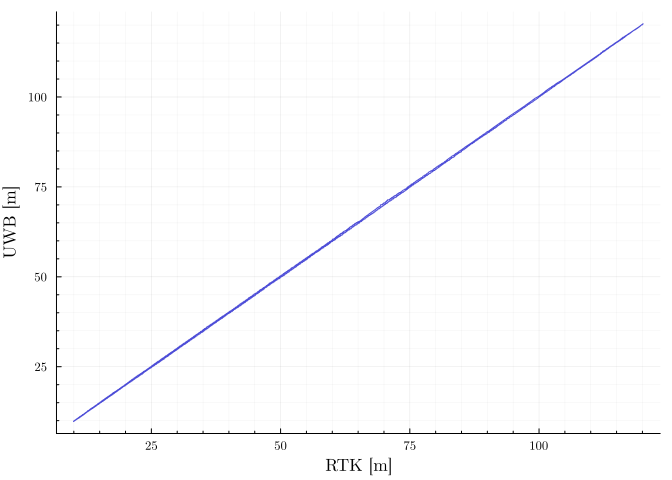
\includegraphics{sections/experiments_files/figure-pdf/fig-tranfer-function-output-1.pdf}

}

\caption{\label{fig-tranfer-function}Transfer characteristic of UWB}

\end{figure}

\begin{figure}

{\centering 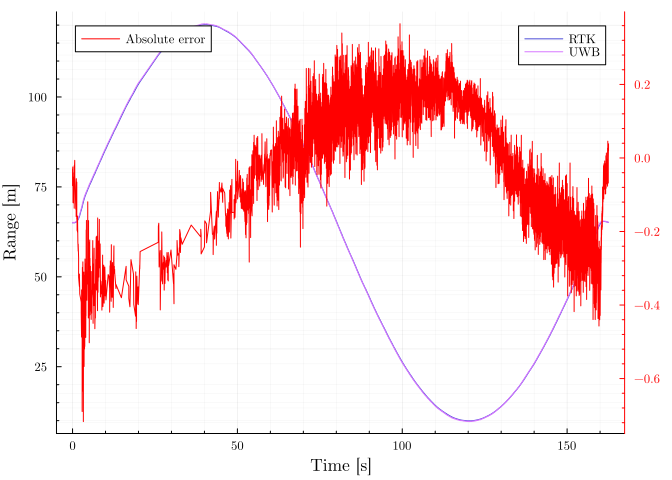
\includegraphics{sections/experiments_files/figure-pdf/fig-line-in-time-output-1.pdf}

}

\caption{\label{fig-line-in-time}Transfer characteristic of UWB}

\end{figure}

\begin{figure}

{\centering 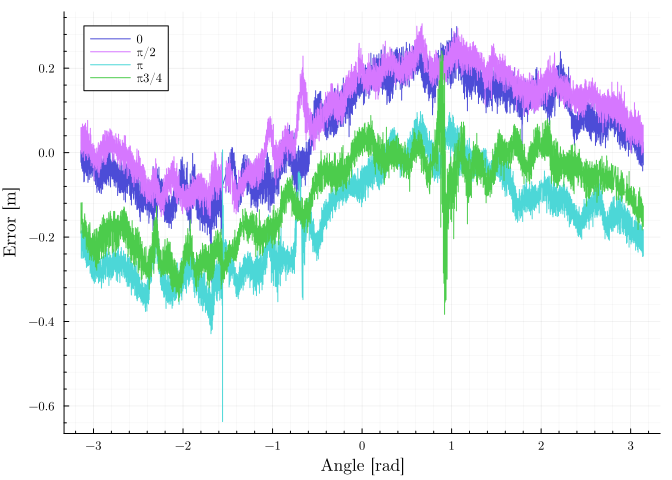
\includegraphics{sections/experiments_files/figure-pdf/fig-angle-output-1.pdf}

}

\caption{\label{fig-angle}Transfer characteristic of UWB}

\end{figure}

\bookmarksetup{startatroot}

\hypertarget{bibliography}{%
\chapter*{Bibliography}\label{bibliography}}

\markboth{Bibliography}{Bibliography}

\appendix

\hypertarget{refs}{}
\begin{CSLReferences}{0}{0}
\leavevmode\vadjust pre{\hypertarget{ref-qorvo:aps011}{}}%
\CSLLeftMargin{1. }%
\CSLRightInline{2014. \emph{A sources of error in DW1000 based two-way
ranging scheme APS011}. Decawave;
\url{https://www.qorvo.com/products/d/da008446}.}

\leavevmode\vadjust pre{\hypertarget{ref-mrs:uvdar}{}}%
\CSLLeftMargin{2. }%
\CSLRightInline{Viktor Walter, Nicolas Staub, Antonio Franchi, and
Martin Saska. 2019. UVDAR system for visual relative localization with
application to leader--follower formations of multirotor UAVs.
\emph{IEEE Robotics and Automation Letters} 4, 3: 2637--2644.
\url{https://doi.org/10.1109/LRA.2019.2901683}}

\end{CSLReferences}

% \medskip

% \appendix

% \printindex

% \appendix

% \bibliographystyle{amsalpha}
% \bibliography{ctutest}

\end{document}
